\chapter{Sampling Distributions and the Central Limit Theorem}
\section*{Chapter 7 Review}

Our first goal in Math 326 is to learn how to estimate global parameters of \say{population} like $\mu$ and $\sigma$. To do this, we need to understand how the random variable we use to estimate them are distributed. For example:
$$
\text{Parameters }\left\{\begin{aligned}
    \mu
    \\
    \sigma^2
\end{aligned}\right.
\hspace{0.5in}\text{Statistics }
\left\{\begin{aligned}
    \Xbar &= \over{n} \sum X_i
    \\
    S^2 &= \over{n-1} \sum \pars{X_i - \Xbar}^2
\end{aligned}\right.
$$

\setSection{1}
\section{Sample Means}

\begin{enumerate}[label=\textcircled{\raisebox{-1pt}{\arabic*}}]
    \item \textbf{Sample means: }
    \addcontentsline{toc}{subsection}{Theorem 7.1}

    \nl\textbf{Theorem 7.1}: Let $\yn$ be a random sample from $\normalDist*$ then $\Ybar$ is distributed by $\normalDist{\mu}{\dfrac{\sigma^2}{n}}$. The distribution of sample means, $\Ybar$, is also Normal.

    \reason* Linearity of Expectation and Variance properties 

    \disc* Recall in working with $\normalDist*$, we learned it was easier to standardize\\everything via
        $Z$-scores: $$Z = \frac{x-\mu}{\sigma}$$
        and $Z$ is distributed $\normalDist{0}{1}$, the \textbf{Standard Normal Distribution.}
        
        
    \item
        \textbf{Sample variance:}
        
        \nl Recall standard deviation $\sigma$ is a measure of the spread of the random variable and it's derived from $\pars{Y_i - \Ybar}^2$ terms. In all math, we normalize to take the \say{units} out of things.
        $$\underbrace{U_i = \frac{Y_i - \bar{Y}}{S}}_{\text{Data Driven = Stat}} \approx \underbrace{\frac{Y_i - \mu}{\sigma} = Z_i}_{\text{Not a stat}}$$
        
        \reason* $Z_i$ depends on unknown population parameters, nonetheless, it makes it easier to pretend that we start here.

        \addcontentsline{toc}{subsection}{Theorem 7.2}
        \nnl
        \textbf{Theorem 7.2} If $\yn$ are a random sample of $\normalDist*$. Then,
        $$U = \sum Z_i^2 = \sum \pars{\frac{Y_i - \mu}{\sigma}}^2$$
        has a $\chi^2$ distribution with $n$ degrees of freedom (df).

        \nl
        \textit{Recall}: $\chi^2$ distribution is a $\gammaDist{\dfrac{\nu}{2}}{2}$ where $\nu = \df$ (degrees of freedom).

        \reason In old homework (325), ${Z_i}^2$ is $\chi^2$ with $\df = 1$.
        By product of mgf, $\sum {Z_i}^2$ is $\chi^2$ with $\df = n$. Now to get sample variance, we do some algebra:
        \notab{\begin{align*}
            && S^2 &= \frac{1}{n-1}\sum(Y_i-\bar{Y})^2 \\
            &&& \approx \frac{1}{n-1}\sum(Y_i - \mu)^2 \\
            \iff && \frac{S^2}{\sigma^2} &\approx \frac{1}{n-1}\sum \pars{\frac{Y_i - \mu}{\sigma}}^2\\
            \iff && \frac{S^2(n-1)}{\sigma^2} &\approx \sum {Z_i}^2
        \end{align*}}

        \nl Showing it is okay to replace $\Ybar$ with $\mu$ is the point of the proof of the following theorem:

        \addcontentsline{toc}{subsection}{Theorem 7.3 (Fisher's Theorem)}
        
        \nnl \textbf{Theorem 7.3 (Fisher's Theorem)} The distribution of sample variance $S^2$

        \nl If $\yn$ is a random sample from $\normalDist*$. Then,
        \begin{enumerate}[label=\textcircled{\raisebox{-1pt}{\arabic*}}]
            \item 
                $\dfrac{S^2(n-1)}{\sigma^2}$ has $\chi^2$ distribution with $(n-1)$ degrees of freedom.
            
            \item
                $\bar{Y}$ and $S^2$ are independent random variables.

        \end{enumerate}

                    
        \item
        $t$-distribution and $F$-distribution
        $$\underbrace{\frac{Y_i-\mu}{\sigma}}_{\text{Normal}} \approx \underbrace{\frac{Y_i -\mu}{S}}_{\text{t-dist'n}} \approx \underbrace{\frac{Y_i - \bar{Y}}{S}}_{\text{Statistic}}$$

        \nl Address when to use what is the point of this class

        \nl Skip definitions (such as moments) for the time being

        \nl Also, The Law of Large Numbers. Used to prove the Central Limit Theorem.
\end{enumerate}








\newpage
\setSection{3}
\section{The Central Limit Theorem}

The reason Normal distributions play an outsized role in applied statistics is that the distribution of  $\bar{Y}$ can be made \emph{nearly normal}, no matter the underlying distribution of $Y$ (Does not need to start \say{life} Normal). So \emph{nearly} normal, that we just pretend it is.



\nnl \textbf{Theorem 7.4: The Central Limit Theorem (CLT)}

\nl Let $\yn$ be independent and identically distributed (iid) random variables with
$$\E{Y_i} = \mu \wideand \Var{Y_i} = \sigma^2 < \infty$$
(Need finite variance for CLT to hold)

\nl Define $$U_n = \frac{\bar{Y}-\mu}{\sqrt{\frac{\sigma^2}{n}}} = \frac{\sum (Y_i) - n\mu}{\sigma \sqrt{n}}.$$

\nl The CLT says the distribution function of
$U_n$ converges to $N(0,1)$ as $n\to\infty$.

\nl Big idea: The distribution $\Ybar$ can be thought of as $\normalDist{\mu}{\frac{\sigma^2}{n}}$.

\defn The \bu{support of $f$} is the domain on which $f$ is non-zero.

\example* Let $\Xbar$ denote the mean of a random sample of size $n=15$, from the distribution whose pdf is $$f(x) = \frac{3}{2}x^2, \qquad x \,\in\, [-1,1]$$


\nl Can be shown that
$$\mu = \Eb{X} = 0 \wideand \sigma^2 = \Eb{(X-\mu)^2} = \frac{3}{5}$$

\nl To compute $\P{0.03 \leq \Xbar \leq 0.15}$, we use the CLT and assume $\Xbar$ is distributed  by
$$\normalDist{\mu}{\frac{\sigma^2}{n}} = \normalDist{0}{\frac{3/5}{15}} = \normalDist{0}{\over{25}}.$$

\nl Then
\begin{align}
    \P{0.03 \leq \bar{X} \leq 0.15} &= \P{\frac{0.03-\mu}{\sigma} \leq \frac{\Xbar - \mu}{\sigma} \leq \frac{0.15-\mu}{\sigma}} \notag\\
    &= \P{\frac{0.03-0}{\sqrt{1/25}} \leq Z \leq \frac{0.15-0}{\sqrt{1/25}}} \notag\\
    &= \P{\frac{0.03}{\sqrt{1/25}} \leq Z \leq \frac{0.15}{\sqrt{1/25}}} \notag\\
    &= \P{0.15\leq Z \leq 0.75} \notag\\
    &= \text{Table4}(0.15) - \text{Table4}(0.75)\notag\\
    &= 0.4404 - 0.2266 \notag\\
    &= 0.2138 \notag
\end{align}
\recall Table 4 gives \underline{upper} tail probabilities.

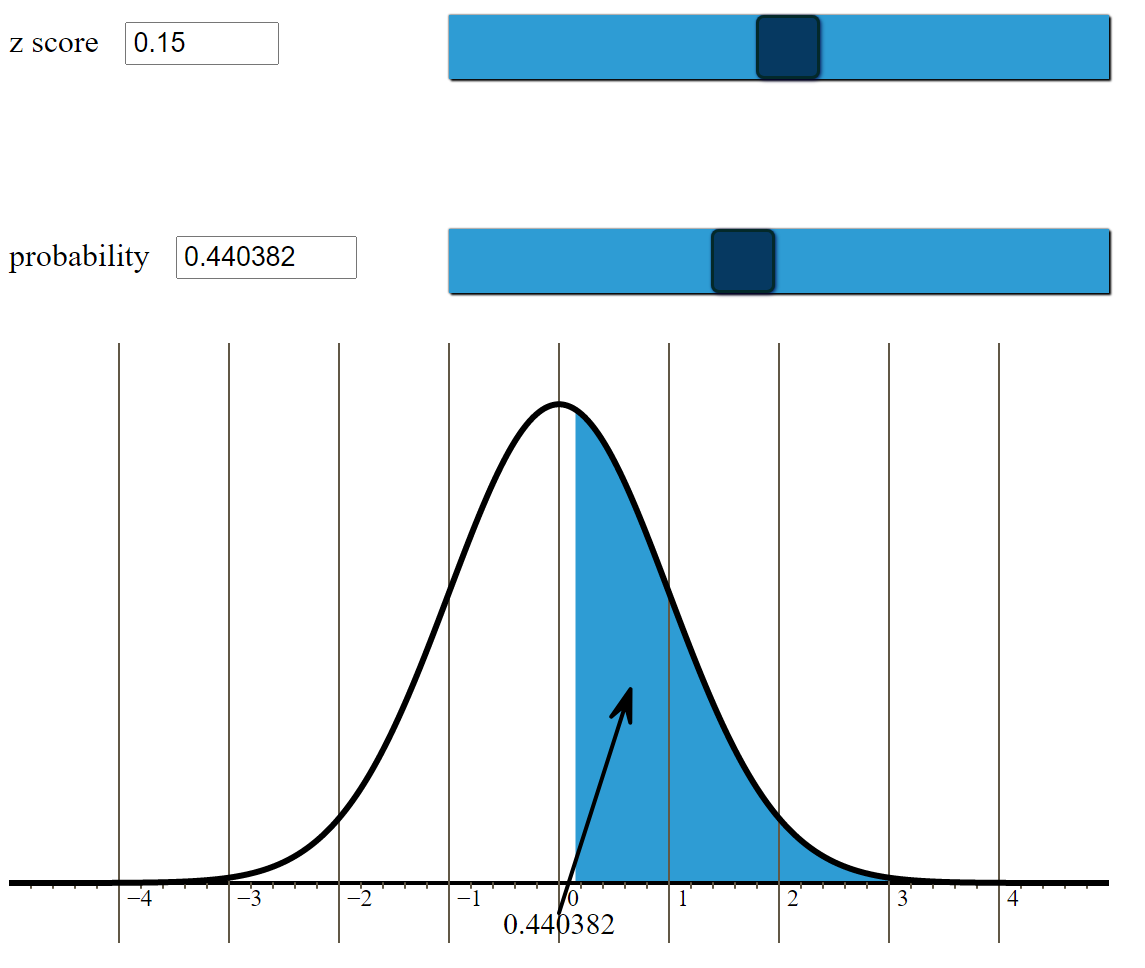
\includegraphics[width=3in]{z 0.15.PNG}
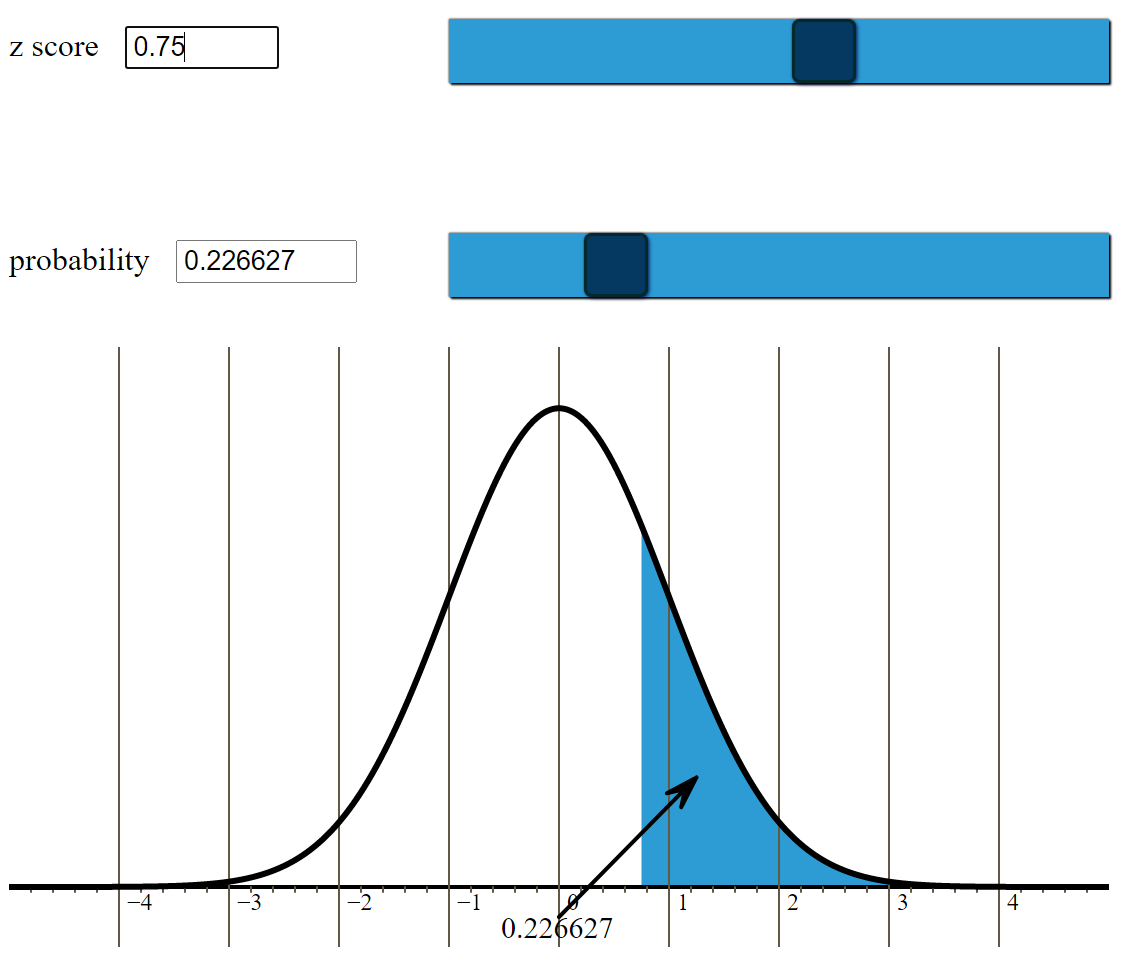
\includegraphics[width=3in]{z 0.75.PNG}

\nl Therefore, 
\begin{align*}
    \text{Table4}(0.15) - \text{Table4}(0.75) &= \P{Z > 0.15} - \P{Z > 0.75}\\ &= 0.4404 - 0.2266 \\ &= 0.2138
\end{align*}

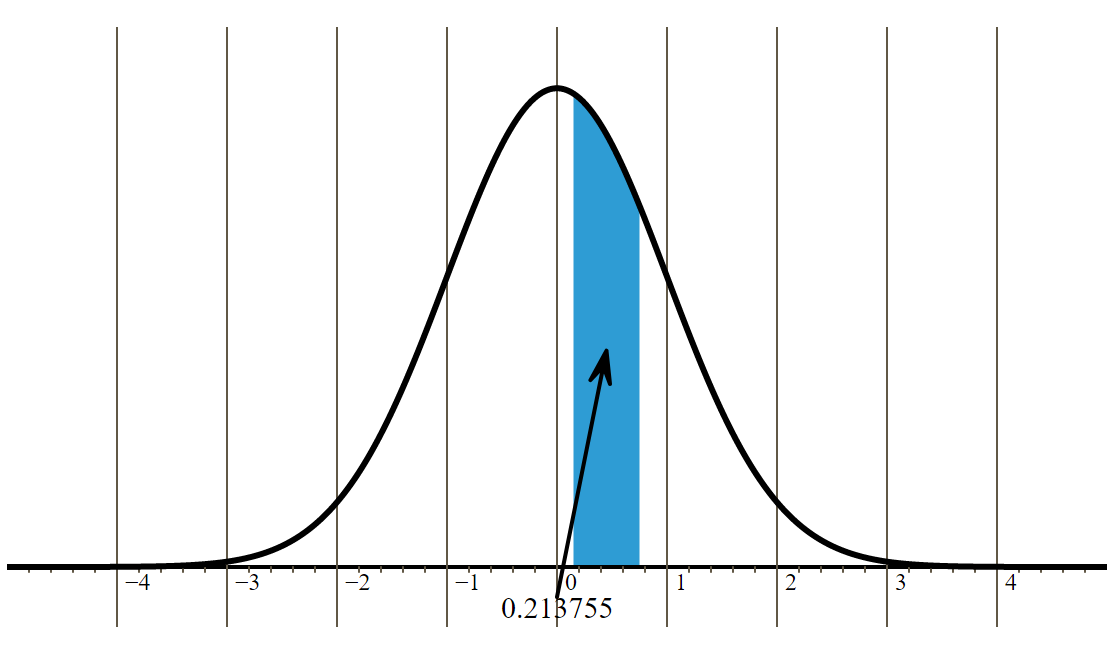
\includegraphics[width=6.25in]{7_4 normal area.PNG}

\disc* About $n$. Suprisingly, \say{large} $n$ doesn't need to be that large.\\Usually for any random variable $X$ and any distribution, then
$$\boxed{n \geq 30 \quad \text{is enough.}}$$

\noindent
That is, when $n \geq 30$, the CLT says $\normalDist{\mu}{\frac{\sigma^2}{n}}$ yields a good approximation of $\Xbar$.

\nl When $X$ is symmetric, unimodal, and continuous, $n = 4$ or $n = 5$ is often enough. 

\newpage
\addcontentsline{toc}{subsection}{Table 4: Normal Curve Areas}
\noindent\begin{center}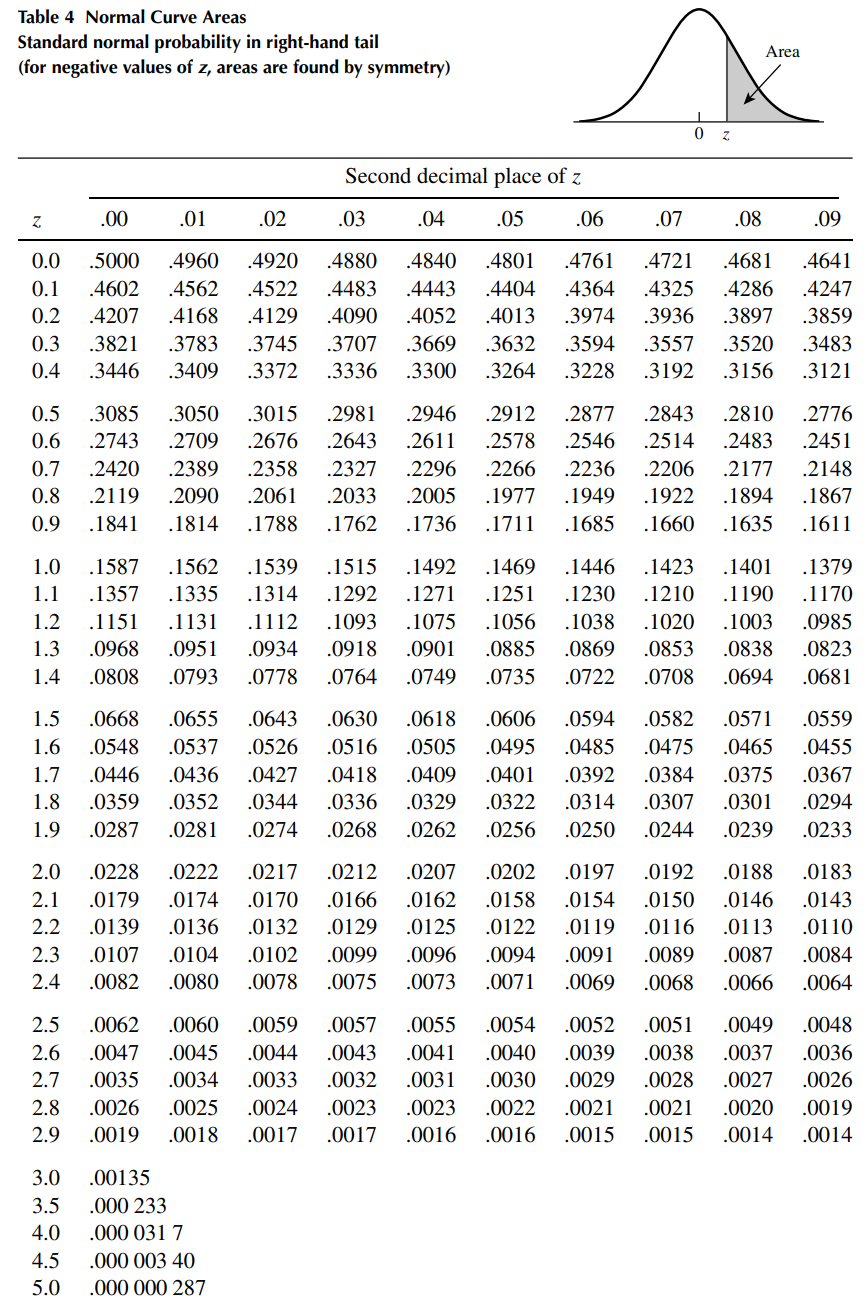
\includegraphics[width=6in]{Table4.png}
\end{center}